\subsection{Energy Improvement from MCRP}

%There have been various studies to estimate the nodes energy consumption in real time in order to prolong the network lifetime. There are two main ways that are usually studied for an energy-efficient WSN which are through MAC and routing protocols. In MAC protocols, the radio duty cycle is exploited to minimise the radio usage which as a result, enable the nodes to be awake efficiently for transmission or reception without wasting energy idling.
%In term of the routing protocols, nodes load have to be fairly spread to use different nodes during communication. This is because nodes that are closer to the sink are the most constrained. Those nodes have more traffic to forward which resulted in more bandwidth and energy being used than the other nodes. 

%Another important factor that effects the energy consumption that has been extensively studied through MCRP processes in this thesis is the condition of the radio link. By using reliable radio channel, retransmission could be avoided. 
Multichannel protocol not only could reduce the end to end delay, it also helps to improve the nodes energy efficiency by ensuring minimal packet retransmissions thus energy consumption.
MCRP implements Contiki's existing energy module, Powertrace.
%Most solutions that estimate the nodes energy consumption use metrics such as the radio duty cycle and end to end delay to represent the energy consumption. One of the reasons for this is the energy consumption estimation is often used to compare among different nodes thus the voltage is not required to be computed. It is possible to measure the battery level for the battery powered sensors. However, it cannot be directly translated for energy estimation because the voltage level of the battery does not linearly translate to the amount of remaining lifetime.
%This chapter describes the implementation of Contiki existing energy module. It also shows the energy consumption estimation computation and the implementation in MCRP. The energy consumption in MCRP is evaluated in term of the end-to-end and forwarding packets energy. The results showed that MCRP consumes less energy than a single channel with interference.
Powertrace uses the software based on-line energy estimation mechanism \cite{dunkels2007software} to estimate the node's current energy consumption in real time. 
%The on-line energy estimation is implemented in Contiki OS. 
The energy estimation module uses time measurements that can be directly obtained from the microprocessor on-chip timer when the component is switched on to produce a time stamp. The time difference from when the component was on and when it later is switched off is computed. The current draw of the component listed in the TelosB data sheet is used to compute the total energy consumption estimation. 

\begin{equation}
E = (I_{m}t_{m} + I_{l}t_{l} + I_{tx}t_{tx} + I_{r}t_{r} +  \sum_{i}I_{c_{i}}t_{c_{i}}) \times\frac{V}{32768}
\label{energyModel}
\end{equation}

Equation \ref{energyModel} shows the energy consumption model given in \cite{dunkels2007software}, $E$ in $mJ$ where $V$ is the supply voltage, $I$ the current draw and $t$ the active time computed in Powertrace for $m$ the microprocessor, $l$ the microprocessor in low power mode, $tx$ the communication device in transmit mode, $r$ the communication device in receive mode and $c_{i}$ for other components such as sensors and LEDs. The values of $I_{m}$, $I_{l}$, $I_{tx}$ and $I_{r}$ are device dependent. In this paper, $I_{m}$ is $1.8 mA$, $I_{l}$ is $0.0545 mA$, $I_{tx}$ is $19.5 mA$ and $I{r}$ is $21.8 mA$. The on-chip timer has the value of $32768Hz$.
%Throughout this thesis, Equation \ref{energyModel2} is used giving the total energy $E$ in $mJ$, the current in $mA$ and $32768Hz$ is the on-chip timer for one second runtime on a $3V$ sensor.

%\begin{equation}
%E = (1.8t_{m} + 0.0545t_{l} + 19.5t_{tx} + 21.8t_{r}) \times \frac{3}{32768}
%\label{energyModel2}
%\end{equation}

%??These energy consumption estimation solutions can be used to improve the network by using the information to reconstruct the topology.

%%ContikiMAC \cite{contikimac} radio duty cycling uses a transmission phase-lock optimisation to significantly reduce the length of a packet transmission. In the beginning, the sender sends the same packet repeatedly to the neighbour until it receives a link layer acknowledgement. The link layer acknowledgement is used as the indicator of the receiver's wake up phase. In the next transmission, the number of the transmissions will be shorter as the sender will send the packet just before the neighbour is expected to be awake based on the neighbour's wake up phase knowledge that it acquired previously. This ensures transmission efficiency which as a result, reduces the network energy consumption thus less radio congestion. 

Powertrace is used to compute the energy consumption estimation of the network. However, the nodes do not have enough capability to compute their individual energy consumption. In order to estimate the energy taken from the sender to the receiver, each node sends their energy values to LPBR regularly as MCRP has a centralised controller. This enables LPBR to predict the energy drain if the routes have high interference or packet losses. LPBR is able to compute the end to end energy consumption on each routes and estimate the nodes battery level based on the energy values. Each node sends the energy value of its packet transmission, packet forwarding and total time value that the radio has been on from the beginning to LPBR for energy consumption computation.
%LPBR has the knowledge of the whole topology.
%Each node accesses only the current entry for it's packet transmission energy and forwarding energy and sends the values to LPBR to compute the energy consumption. 
By doing that, the nodes knowledge of its energy level is kept at minimum. 

%????In future work, LPBR will use these information to reconstruct the topology based on the energy level of each node in prolong the network lifetime.

In order to calculate accurate energy consumption for specific packet transmission, the unicast packet type is separated into normal unicast and control messages unicast. The unicast packet from the application layer (normal unicast) is set as \textit{unicastMsg = 1}, which the value is 0 by default to represents other unicast packets. This allows the energy of the transmission packet to be calculated separately without including other control messages that could be sent right after or before the normal packet transmission. This is done to avoid inaccurate energy spent as control messages are only being sent periodically unlike the normal packet that are sent frequently. It also enables retransmit packets to be included as the current transmission packet energy. This will alert the LPBR on the current condition of the node with much higher energy consumption than the usual energy per packet because of the retransmissions. The $unicastMsg$ value is reset when the link layer acknowledgement is received or the maximum number of retransmission is reached. 

%\begin{figure}
%\centering
%\includegraphics[trim=2cm 2cm 13cm 2cm, clip=true, totalheight=0.45\textheight, angle=270]{implementationFigures/totalE.pdf}
%\caption{Transmission energy consumption}
%\label{fig_txEnergy}
%\end{figure}

%%Figure \ref{fig_txEnergy} shows an example of the $energest$ values that are sent from the transmitting node (node 5) to LPBR which are the transmission $txE_n$, forwarding $fwdE_n$ and total time $totalE_n$ since it first booted to give the information of the total energy that has been used. LPBR receives and keeps the values to calculate the energy consumption in a temporary table. As the network topology might change over time, LPBR has to check the end to end routes before it can calculate the end to end energy consumption for a packet transmission. MCRP does not hardcode the routes because of this reason. However, LPBR keeps the information of each node next hop route which is updated when there are changes. LPBR has the knowledge of the whole topology.
%Algorithm \ref{energy_algo} shows the pseudo-code of the implemented energy consumption calculation processes. The end to end routes are checked each time before the energy consumption is calculated.

%\begin{algorithm}
%\caption{Pseudo-code for LPBR energy consumption}
%\label{energy_algo}
%\begin{algorithmic}[]
%\\\textbf{Notations}
%\\$R$ is a node that is a Route
%\\$txE$ is the transmission period
%\\$fwdE$ is the forwarding period
%\\$totalE$ is the total run time
%\\\textbf{Pseudo-code}
%\\Check which node energy consumption to calculate
%\\Generate the end to end routes taken by the node
%	\State check $R$ $currentCh$
%	\If{next hop node $=$ $R$}
%		\State $R$ is node next hop
%		\State check $R$ next hop
%		\If{$R$ $=$ $LPBR$}
%			\State all end to end routes found
%			\State access energy table node $txE$, $R$ $fwdE$
%			\State compute energy consumption using Equation %\ref{energyModel2}
%		\EndIf
%	\Else
%		\State check $R$ next hop $R$
%		\State update the routes
%	\EndIf
%\EndIf
%\end{algorithmic}
%\end{algorithm}
 
%In the example, the total transmission energy consumption for node 5 is the sum of $txE_{5}$ and the $\sum_{i=2}^{4} fwdE_i$ of all the hops before reaching the LPBR. The $fwdE_n$ is the node transmission energy consumption that is used when it only forwards the packet. It is kept separately from $txE_n$ to avoid confusion when the node n is transmitting its own packet after forwarding the other node's packet as the $energest$ values might vary. Equation \ref{energyModel2} is used to calculate the energy consumption in $mJ$.

\subsection{Energy Performance Evaluation}

%This section describes the evaluation of the energy consumption as the result of the proposed multichannel protocol. The performance of MCRP is evaluated using the end-to-end energy, the energy consumption over time and the forwarding packets energy.

%Using the simulation layout as shown in Figure \ref{fig_simulation}, 
The energy consumption in MCRP in term of transmission per packet, forwarding packets energy and total energy used are computed to prove that multichannel helps to prolong the network lifetime by using the energy more efficiently than in a single channel network. Each node sends one packet per minute, 350 packets in total throughout the simulation period. Equation \ref{energyModel} is used to calculate the nodes energy consumption. The energy consumption of each node is computed by the LPBR based on the information contained in the transmitted packet. The maximum number of hops in the simulation is 3 hops. The results of a single channel with no interference is used as the base case as it is the ideal energy consumption value. The results are also compared to the energy of a single channel with moderate and extreme interference, and MCRP for multi channels.

%Node 2, 5 and 15 energy usage are selected for comparisons as other nodes show similar result. Node 2 is one hop to LPBR while node 5 is 2 hops and node 15 is 3 hops away. 

\subsubsection{Energy Per Packet Performance}

\begin{figure}
\centering
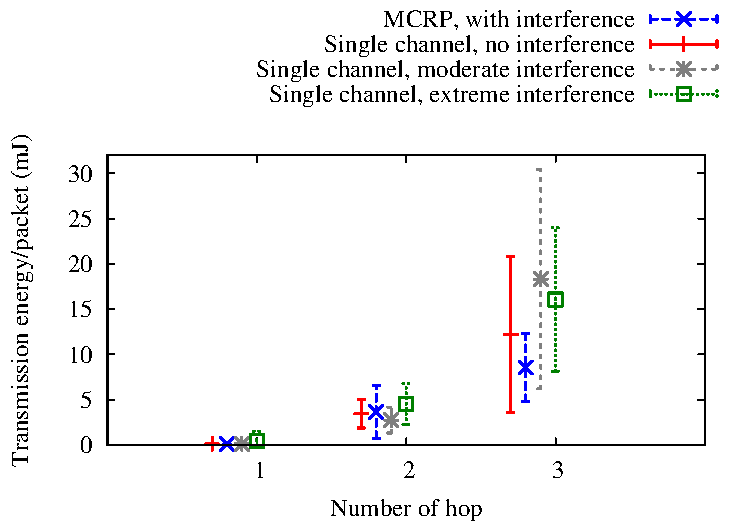
\includegraphics[width=0.45\textwidth]{figures/perPktEnergy.pdf}
\caption{The energy consumption per packet in different number of hops}
\label{fig:energyPerPkt}
\end{figure}

%\begin{figure}
%\centering
%\subfigure[Node 2 energy consumption]{\label{fig:2perPkt}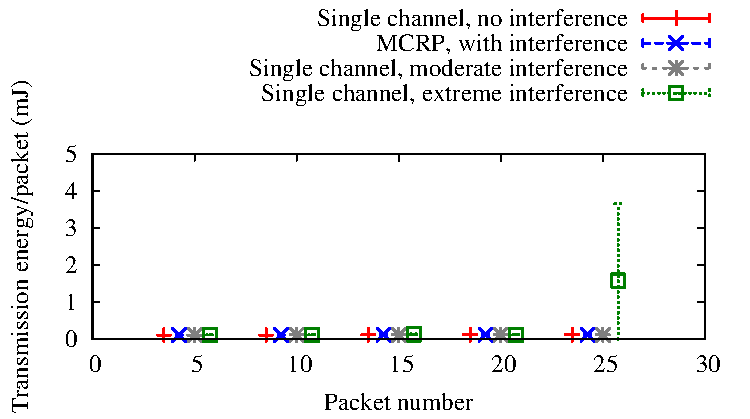
\includegraphics[width=0.45\textwidth]{figures/2EnergyPerPkt.pdf}}                
%\subfigure[Node 5 energy consumption]{\label{fig:5perPkt}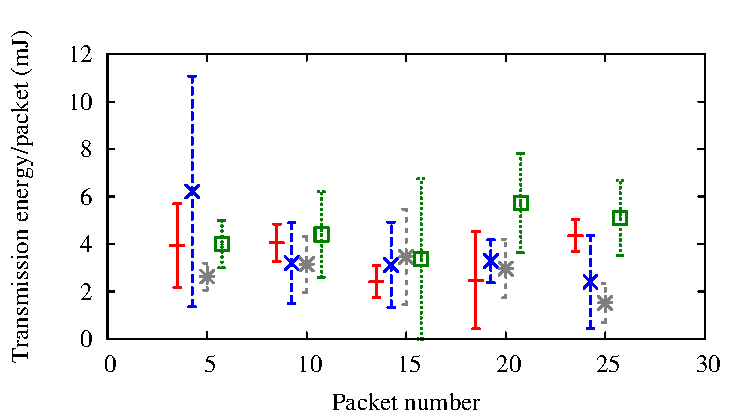
\includegraphics[width=0.45\textwidth]{figures/5EnergyPerPkt.pdf}}
%\subfigure[Node 15 energy consumption]{\label{fig:fperPkt}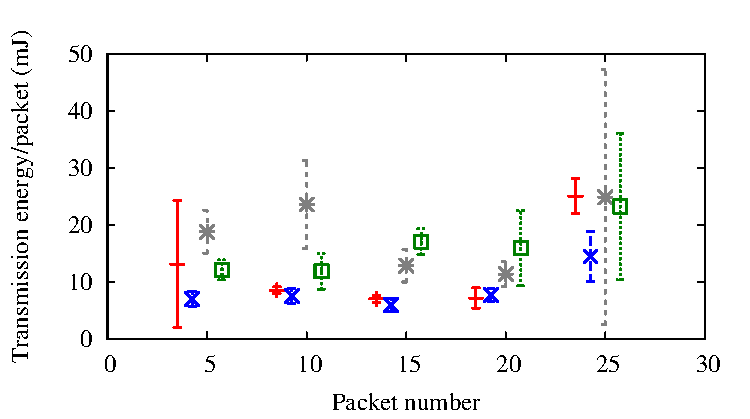
\includegraphics[width=0.45\textwidth]{figures/fEnergyPerPkt.pdf}}
%\caption{Comparison of energy consumption per packet for node 2, 5 and 15}
%\label{fig:energyPerPkt}
%\end{figure}

Figure \ref{fig:energyPerPkt} shows the transmission energy per packet for nodes that are 1, 2 and 3 hops away from the LPBRs. From the figure, it can be concluded that less transmission energy is used when there is less number of hops. However, in a large scale network, the number of hops cannot be reduced as not all nodes would be in the range or directly connected to the destination node. Thus, the node's next hop should be selected carefully to avoid nodes that have higher interference rate.

In the 1 hop case, it can be seen that the nodes consumed approximately similar energy in all cases. As the nodes are one hop to the destination (LPBR), it was not affected by the interference except for a slight variation in the single channel with extreme interference case. 
%Node 3 gives similar result to node 2 as it is also one hop to the LPBR. 
%Figure \ref{fig:5perPkt} and Figure \ref{fig:fperPkt} show higher values of energy that a packet requires from the sender (node 5 and 15) to LPBR through 2 and 3 hops. 
Nodes that are 2 and 3 hops away show higher values of per packet energy transmission.
This is because of the interference near to the nodes. The nodes are unable to detect the exact wake-up time for the nodes thus, the nodes have to transmit in a longer period to ensure the packet gets transmitted. In the one hop graph, the energy can be kept at minimum because the LPBR is always awake to accept packet as it is fully powered unlike the other nodes that have to switch the radio off when there are no transmissions and receptions taking place to save the energy.

In the 1 and 2 hops, MCRP shows approximately similar transmission energy consumption to the base case. 
%The transmission energy for a single channel with moderate and extreme interference is slightly higher compared to MCRP in 2 hops. 
In 3 hops, the energy per packet in the single channel with moderate and extreme interference are much higher than the energy used by the base case and MCRP. This shows that the energy per packet depends on the number of hops and the interference that affect the routes. Multichannel helps to mitigate the effect of interference, thus reducing the transmission energy taken to send a packet especially when there are several hops involved.

%\subsubsection{Energy Over Time Performance}
\subsubsection{Total Energy Consumption}

\begin{figure}
\centering
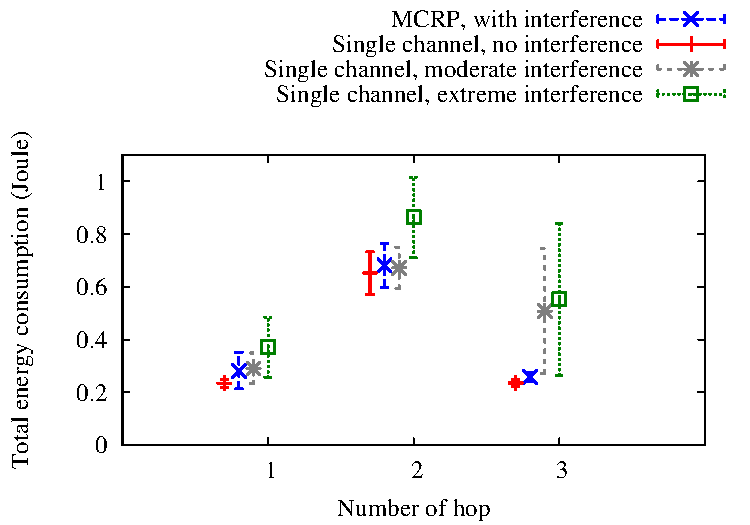
\includegraphics[width=0.45\textwidth]{figures/totalEnergy.pdf}
\caption{Simulation nodes total energy consumption}
\label{fig:allNodesEnergy}
\end{figure}

%\begin{figure}
%\centering
%\subfigure[Node 2 energy consumption]{\label{fig:2total}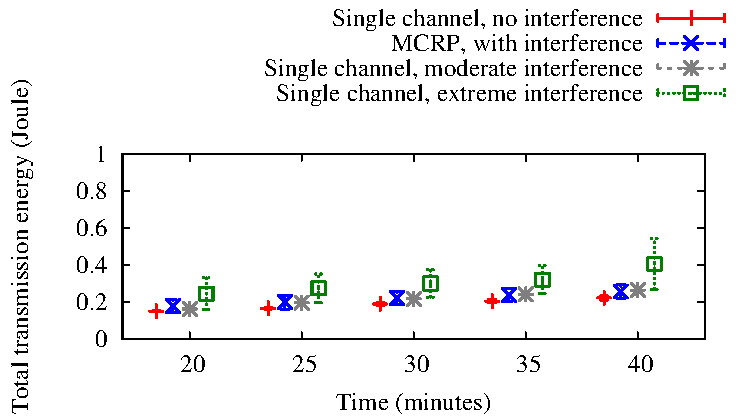
\includegraphics[width=0.45\textwidth]{figures/2Energy.pdf}}      
%\subfigure[Node 5 energy consumption]{\label{fig:5total}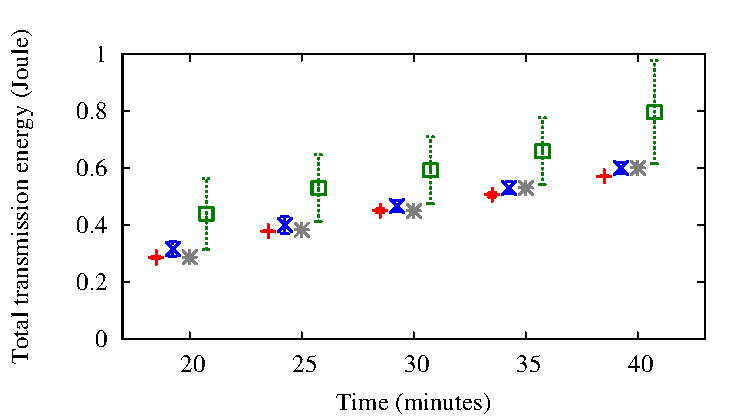
\includegraphics[width=0.45\textwidth]{figures/5Energy.pdf}}          
%\subfigure[Node 15 energy consumption]{\label{fig:ftotal}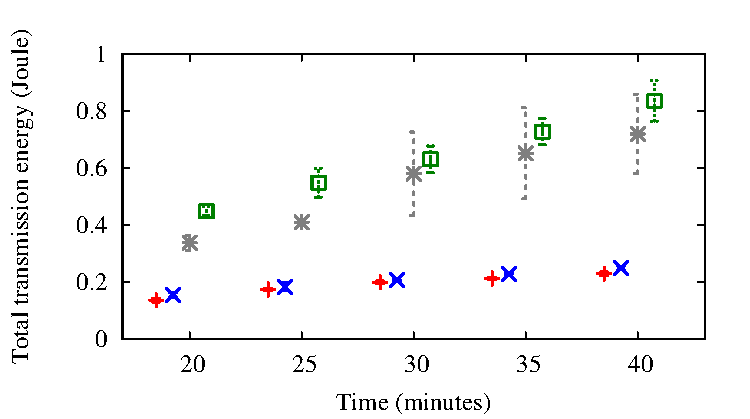
\includegraphics[width=0.45\textwidth]{figures/fEnergy.pdf}}
%\caption{Comparison of total energy consumption for node 2, 5 and 15}
%\label{fig:energyTotal}
%\end{figure}

%Figure \ref{fig:energyTotal} shows the graphs of the three nodes total energy consumption that the nodes took to send 25 packets (approximately 40 minutes) including retransmissions and control packets energy. Figure \ref{fig:2total} shows node 2 energy consumption where it can be seen that in all cases, the total energy taken are approximately similar with a small increase over time. The single channel with extreme interference case however, requires more energy consumption than in other cases. Figure \ref{fig:5total} shows higher increase in energy usage over time in all cases. The reason for this is because node 5 has 2 other nodes that are using it as a forwarder. Node 5 (2 hops) uses higher energy when forwarding packet to LPBR compared to node 2 (1 hop). Figure \ref{fig:ftotal} shows lower energy consumption for node 15 compared to node 5 because node 15 does not act as a forwarder.

Figure \ref{fig:allNodesEnergy} shows the total energy consumption in the simulation including retransmissions and control packets energy. 
%Node 2 and node 3 are one hop to LPBR, nodes 4-7 are 2 hops, and other nodes are 3 hops away. 
In 1 hop, it can be seen that in all cases, the total energy taken are approximately similar with a small standard deviation. The single channel with extreme interference case however, requires higher energy consumption than in other cases.
In 2 hops, it shows high increase in energy usage. The reason for this is because the 2 hops nodes are used as forwarding nodes. The 3 hops nodes do not act as forwarding nodes thus the reason for the lower total energy consumption.
%%%FWD EXPLANATION - The 1 hop nodes consumed less energy than a 2 hops nodes even though the nodes are also acting as forwarders because the LPBR is always on and ready to accept the packets at any time unlike in the 2 hops where the intermediate nodes need to be awake. 
%Node 5 (2 hops) uses higher energy when forwarding packet to LPBR compared to node 2 (1 hop). Figure \ref{fig:ftotal} shows lower energy consumption for node 15 compared to node 5 because node 15 does not act as a forwarder.
The energy consumption is improved when using MCRP than a single channel with interference. This improvement can be clearly seen in the 3 hops nodes as these nodes use more energy during interference for retransmissions. If the retransmissions fail, the packet is dropped and the energy used during the retransmissions is wasted. The total energy consumption graph shows all energy spent when the nodes are awake, including forwarding and failed packets transmission.
%from the packet transmission including failed packet energy.

\subsubsection{Forwarding Energy Analysis}

\begin{figure}
\centering
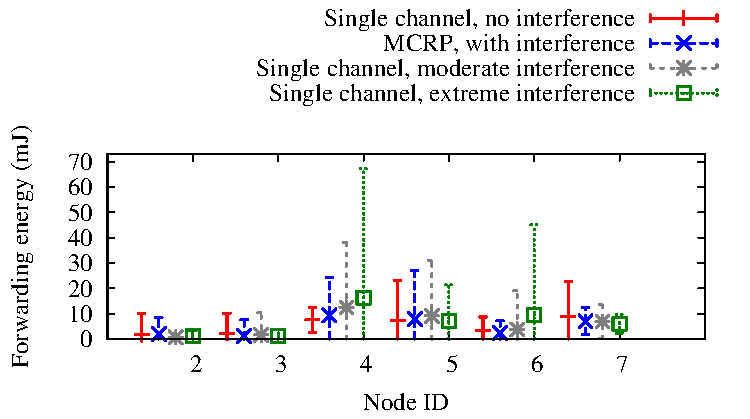
\includegraphics[width=0.45\textwidth]{figures/fwdEnergy.pdf}
\caption{Simulation nodes forwarding energy}
\label{fig:allNodesFwdEnergy}
\end{figure}

Figure \ref{fig:allNodesFwdEnergy} shows the energy used in forwarding packets for the 1 and 2 hops nodes. The 3 hops nodes in the simulation do not forward packets. The 1 hop nodes use less energy than the 2 hops nodes as the nodes only need to check if the channel is being use by the other node before it can forward to the LPBR. LPBR waits for incoming packet thus the nodes could send the packet with less waiting time as LPBR radio is always on. 
%Based on the simulation layout in Figure \ref{fig_simulation}, node 4 and 5 forward packets to node 2 while node 6 and 7 to node 3 as their next hop. Node 4-7 use higher energy than node 2 and 3 in forwarding packets as the nodes have more packets (from the children) to be forwarded. 
In order to be able to forward the packets, the nodes have to be awake for longer time and ensure the intermediate node is also awake and ready to accept the packets. Thus forwarding could require more energy consumption than an end to end packet transmission. By increasing the number of nodes thus children, the nodes will use more energy in order to forward the packets. The forwarding energy consumption contributes to the most energy used by the nodes. 
%MCRP helps to reduce the energy consumption which can be seen in node 4 and 6 results than in a single channel. 
Even though MCRP does not show a lot of improvement, it shows lower deviation compared to the single channel with extreme interference.
In the base case, the energy consumption varies as the nodes are interfering with each other even without external interference during transmissions.

%/////

%This chapter presents the estimated energy consumption calculation. Contiki implemented Powertrace which is a software based energy estimation. MCRP uses Powertrace which tracks the duty cycle and uses the values to measure the estimated energy consumption. 
The simulation results showed that MCRP consumes less energy than in other cases when there is interference as the effect of multichannel. MCRP has similar energy consumption values as in the base case, a single channel without interference. This shows that multichannel helps to reduce the energy wasted due to interference. In order to increase the energy efficiency thus network lifetime, MCRP needs to reconstruct the topology based on the energy consumption, residual energy of the nodes and the link conditions gradually to avoid breaking any current connectivity.
%The next chapter explains MCRP tree optimisation in details.
